% ============================================================================
\section{Results}\label{sec:results}
% ============================================================================

Of 4,976 planned loads, 119 (on 38 stores) were unusable (Supplementary Table~\ref*{S:tab:s-failures}); 23 stores looked like bot blocking, which we did not try to get around. After the 4 stores excluded for content sensitivity (Section~\ref{sec:method-sample}), 1,358 of the remaining 1,396 main-sample stores and all 34 creator stores were captured in all three base arms. Table~\ref{tab:headline} collects the headline estimates.

\begin{table}[!tbp]
\centering
\caption{Headline estimates (main sample unless marked; unweighted). CI: Wilson 95\% interval; for rows marked $^\dagger$ the cluster bootstrap by consent tool is given in brackets. ``Sandboxed'': sent from a Shopify STRICT worker, a LAX iframe or a frame nested in one; a request is a data beacon or a library load. Last row: paired difference in percentage points (pp) with Newcombe's interval.}
\label{tab:headline}
\footnotesize\setlength{\tabcolsep}{4pt}
\begin{tabularx}{\linewidth}{@{}>{\raggedright\arraybackslash}Xrrl@{}}
\toprule
Statistic & $k$/$n$ & \% & 95\% CI \\
\midrule
\multicolumn{4}{@{}l}{\emph{Before any choice (Default)}}\\
Consent banner shown & 409/1,358 & 30.1 & 27.7--32.6 \\
Sandboxed ad request, all stores$^\dagger$ & 803/1,358 & 59.1 & 56.5--61.7 [55.7--62.3] \\
Sandboxed ad request, banner stores$^\dagger$ & 205/409 & 50.1 & 45.3--54.9 [32.6--58.9] \\
\quad default ``allowed until choice''$^\dagger$ & 165/235 & 70.2 & 64.1--75.7 [63.0--79.1] \\
\quad default ``denied until consent''$^\dagger$ & 40/167 & 24.0 & 18.1--31.0 [16.5--36.3] \\
\quad \quad pixel not declaring marketing & 32/167 & 19.2 & 13.9--25.8 \\
First sandboxed request $>$1 poll before banner & 108/205 & 52.7 & 45.9--59.4 \\
\midrule
\multicolumn{4}{@{}l}{\emph{Blocked on paper: declared vendor fired from the sandbox}}\\
CMP wrote no ``yes'' (primary), both samples & 46/89 & 51.7 & 41.5--61.8 \\
\quad main sample & 7/14 & 50.0 & 26.8--73.2 \\
\quad expansion, ranks 200k--1M & 39/75 & 52.0 & 40.9--62.9 \\
All blocklist stores, both samples & 67/117 & 57.3 & 48.2--65.9 \\
Configured sandboxed pixel of that vendor & 10/15 & 66.7 & 41.7--84.8 \\
CMP told Shopify ``marketing: no'': sandboxed request & 39/65 & 60.0 & 47.9--71.0 \\
\midrule
\multicolumn{4}{@{}l}{\emph{Decline}}\\
No first-layer reject option (banners found) & 165/405 & 40.7 & 36.1--45.6 \\
Refusal recorded (working clicks) & 196/231 & 84.8 & 79.7--88.9 \\
New sandbox fired on the fresh page (working clicks)$^\dagger$ & 53/231 & 22.9 & 18.0--28.8 [17.4--29.5] \\
Any sandboxed request after the click (working clicks) & 80/231 & 34.6 & 28.8--41.0 \\
\midrule
\multicolumn{4}{@{}l}{\emph{GPC}}\\
``Sale of data: no'' (loads with a readable state) & 1,166/1,169 & 99.7 & 99.2--99.9 \\
At-risk loads in which a sale-of-data pixel started & 0/1,264 & 0.0 & 0.0--0.3 \\
Still sending, of stores sandboxed under Default$^\dagger$ & 279/803 & 34.7 & 31.5--38.1 [30.9--38.7] \\
\midrule
Blocklist minus no declaration, both samples (Mantel--Haenszel), pp & & 13.4 & 4.0 to 22.8 \\
Decline minus GPC (53 vs 41 of 231 stores), pp & & 5.2 & 0.2 to 10.3 \\
\bottomrule
\end{tabularx}
\end{table}

% ----------------------------------------------------------------------------
\subsection{RQ1: Sandboxed pixels fire before any choice}\label{sec:res-prechoice}
% ----------------------------------------------------------------------------

Before any click, an ad request left the page on 1,254 of 1,358 stores (92.3\%, 95\% CI 90.8--93.6\%), and a \emph{sandboxed} one on 803 (59.1\%, 56.5--61.7\%). A consent banner appeared on 409 stores (30.1\%), and on half of these a sandboxed ad pixel fired before any choice: 205 of 409 (50.1\%, 45.3--54.9\%; Fig.~\ref{fig:situating}c; per vendor group: Supplementary Fig.~\ref*{S:fig:s6}a), against 598 of 949 stores without a banner (63.0\%, 59.9--66.0\%; Supplementary Fig.~\ref*{S:fig:s6}e). Neither library loads nor missed banners explain this (Supplementary \ref*{S:sec:s-extended}).

\begin{widefig}
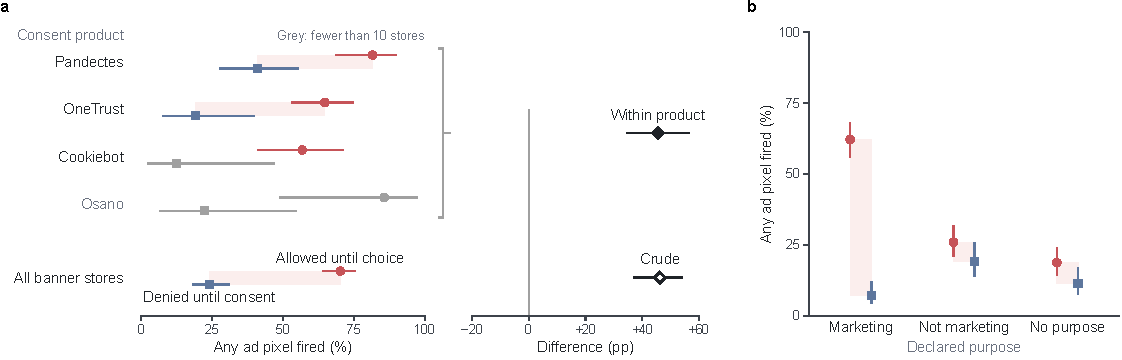
\includegraphics{fig3.pdf}
% GENERATED by paper/integrate_figures_v2.py from figures/v7/fig3/caption_fig3.tex (v2 figure caption, rendered by the figure script).
% Do not edit: change the figure script and re-run build.sh.
\caption{\textbf{Before any choice, whether sandboxed pixels fire tracks Shopify's region default, even within the same consent tool.} (a)~Left: share of banner stores on which an ad pixel running in a Shopify sandbox sent a request before any choice, by Shopify's region default at our California vantage point: `allowed until choice' (brick circles, just above each row's centre line) and `denied until consent' (slate squares, just below it). Rows: the 4 consent-management platform (CMP) products with at least 5 stores under each default, in order of their Mantel--Haenszel (MH) weight; stores that fired / stores, `allowed' then `denied': Pandectes 40/49 and 18/44; OneTrust 44/68 and 4/21; Cookiebot 21/37 and 1/8; Osano 6/7 and 2/9. Bottom row, set apart: all 402 banner stores with a readable default, 165 of 235 (70.2\%; 95\% confidence interval (CI) 64.1--75.7\%) against 40 of 167 (24.0\%; 18.1--31.0\%). A group of fewer than 10 stores is drawn grey, as the note in the plot says (Cookiebot's `denied' group and both of Osano's; a row with no coloured group has its name in grey). Pale brick band: the excess under `allowed until choice', from the `denied' share to the `allowed' share, drawn where both groups are coloured. Right, on the same rows and the same scale: the difference, `allowed' minus `denied', in percentage points (pp), with its 95\% CI (horizontal line), against a grey zero line: pooled within product by the MH method with Sato's variance (filled diamond, `Within product', level with the middle of the product rows, which a grey bracket groups) +45.6~pp (34.6--56.6), and over all banner stores (open diamond, `Crude', on their row; Newcombe's interval) +46.3~pp (36.9--54.3). The pooled difference uses all 12 CMP products with stores under both defaults (354 stores; the other 48 use a product seen under one default only, or none); the 4 drawn on the left carry 84\% of its weight. The other 8, with fewer than 5 stores under one default, are not drawn: Usercentrics 5/6 and 0/3; iubenda 6/8 and 1/2; Ketch 2/2 and 1/5; Clarip 2/4 and 0/2; Shopify's banner 1/1 and 11/65; CookieScript 4/5 and 1/1; CookieYes 4/4 and 0/1; consentmanager 0/1 and 1/1. The 7 banner stores without a readable default are not shown; none of them fired. (b)~The same measure, counting only the pixels that declare a given purpose, with the markers of (a) (brick circles `allowed until choice', slate squares `denied until consent'), its intervals and pale brick bands, and the same scale: `marketing' 146 of 235 (62.1\%) against 12 of 167 (7.2\%); not `marketing' 61 of 235 (26.0\%) against 32 of 167 (19.2\%); no purpose at all (a subset of not `marketing') 44 of 235 (18.7\%) against 19 of 167 (11.4\%). A store can count under more than one purpose. On 11 of the 12 `denied' stores with a firing `marketing' pixel, the CMP had first told Shopify `yes' without a click. Lines through the circles and squares: Wilson 95\% CIs, each in the colour of its mark (stores are the unit). All three plots share one scale (the same length per percentage point). Default load (no interaction); main sample 1,358 stores, 409 with a banner. Per-vendor rates, the timing of the first sandboxed request, request origins and per-product shares: Fig.~S6.}
\label{fig:region-default}

\end{widefig}

Pre-choice firing on banner stores was most strongly associated with Shopify's region default (Fig.~\ref{fig:region-default}a): it occurred on 165 of 235 banner stores (70.2\%, 64.1--75.7\%) where the consent string allowed marketing until the visitor chose, and on 40 of 167 (24.0\%, 18.1--31.0\%) where it denied marketing until consent. This contrast, specified before the crawl (prediction P1), is partly confounded with the consent product but persists within products (Mantel--Haenszel difference over 12 products 45.6 percentage points, 95\% CI 34.6 to 56.6). For pixels that declare marketing, which the gate is meant to hold back, the contrast is sharper, 146 of 235 (62.1\%) against 12 of 167 (7.2\%), and on 11 of those 12 stores the CMP had told Shopify ``yes'' without any click. This is F1: the sandbox follows Shopify's state, and the banner matters only insofar as the CMP changes that state.

The ``denied until consent'' stores are the closest this vantage point comes to an opt-in regime such as the EU's. On 32 of these 167 banner stores (19.2\%, 13.9--25.8\%), a sandboxed ad request before any choice came from a pixel that does not declare marketing, and on 19 (11.4\%, 7.4--17.1\%) from one that declares no purpose at all: an opt-in default does not hold back pixels that do not declare the purpose it withholds (F4).

Because the banner detector polled every 250~ms, a request counts as preceding the banner only if it came more than one polling interval earlier. On 108 of the 205 banner stores with a pre-choice sandboxed request (52.7\%, 45.9--59.4\%), the first request came that early (Supplementary Fig.~\ref*{S:fig:s6}b), and on 151 (73.7\%) before the banner at all; the per-store flag repeated only moderately (Cohen's $\kappa=0.54$ on 46 repeat stores). Where the first request clearly preceded the banner, no choice could have prevented it (Fig.~\ref{fig:situating}c).

The sandbox carried 31.5\% (29.8--33.2\%) of the 40,016 ad requests in Default loads, most for vendors whose app pixels run in STRICT workers (Supplementary Fig.~\ref*{S:fig:s6}c and Table~\ref*{S:tab:s-vendor}).

% ----------------------------------------------------------------------------
\subsection{RQ2: Blocked on paper}\label{sec:res-paper}
% ----------------------------------------------------------------------------

We next asked what happens when a store's consent setup says ``no'' before any choice (Fig.~\ref{fig:blocked-on-paper}; Supplementary Fig.~\ref*{S:fig:s7}). In the main sample, on 21 stores (15 Pandectes, 5 OneTrust and 1 Cookiebot store), a readable blocklist declared at least one ad vendor blocked before any choice. A blocklist is in force only while the CMP has not consented, and on 7 of the 21 the CMP itself wrote ``marketing: yes'' to Shopify without any click, on 2 of them through an optional Pandectes merchant setting that grants consent to automated browsers (Section~\ref{sec:app-validation}). On the other 14 stores the declared-blocked vendor's own pixel sent requests from Shopify's sandbox before any choice on 7 (50.0\%, 26.8--73.2\%).

Fourteen stores give a wide interval, so the expansion crawl (Section~\ref{sec:method-r4}) added 116 stores from ranks 200k--1M, on 96 of which (93 Pandectes, 3 OneTrust) the blocklist was in force at run time. On 21 of the 96 the CMP wrote ``yes'' without a click; on 39 of the other 75 the declared vendor fired from the sandbox (52.0\%, 40.9--62.9\%), a rate no different from the main sample's (difference $-2.0$ percentage points, 95\% CI $-27.6$ to 23.7). Our primary estimate therefore pools the two samples: on 46 of 89 stores (51.7\%, 41.5--61.8\%) a vendor that the blocklist declared blocked sent requests from Shopify's sandbox before any choice, and on 37 (41.6\%, 31.9--52.0\%) it did so from a pixel that declares marketing. Over all 117 blocklist stores the rate was 67 (57.3\%, 48.2--65.9\%); design-weighted and alternative estimates are in Supplementary \ref*{S:sec:s-r4} and~\ref*{S:sec:s-extended}.

\begin{widefig}
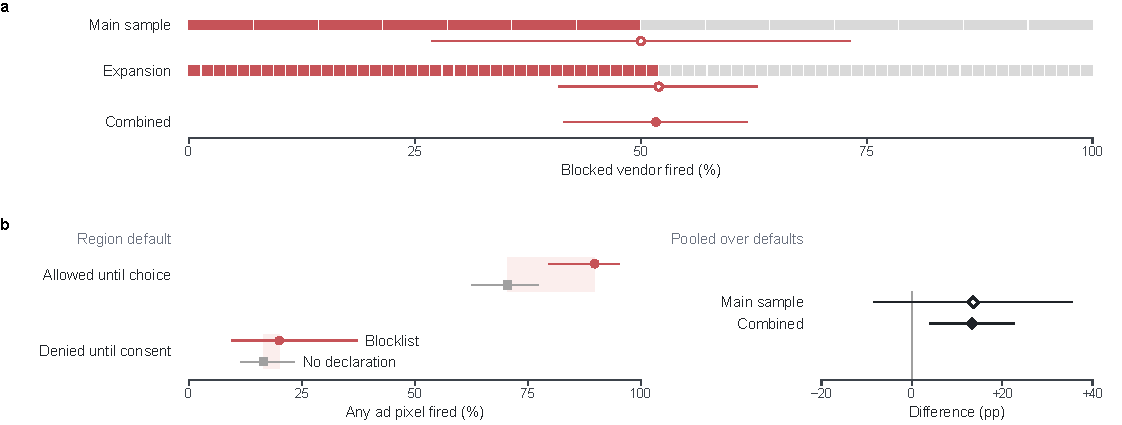
\includegraphics{fig4.pdf}
% GENERATED by paper/integrate_figures_v2.py from figures/v7/fig4/caption_fig4.tex (v2 figure caption, rendered by the figure script).
% Do not edit: change the figure script and re-run build.sh.
\caption{\textbf{Blocked on paper: a vendor that the consent tool's blocklist declares blocked still fired from Shopify's sandbox on about half of the stores, and blocklist stores fired more, not less, often than comparable stores.} (a)~Point~(2) of Fig.~1a at scale: blocklist stores whose consent-management platform (CMP) wrote no `marketing: yes' to Shopify in the Default load (no interaction), and whether the ad vendor that the CMP's blocklist declared blocked sent a request from its sandboxed Shopify pixel before any choice. Each bar is one sample, one cell per store across the full axis: brick cells, the stores on which the declared-blocked vendor fired, drawn first so that the brick part ends at the share; light grey cells, the stores on which it did not. Under each bar, the sample's share (open circle) with its 95\% confidence interval (CI): main sample (Tranco top 200,000) 50.0\% (7 of 14), expansion 52.0\% (39 of 75). Below a gap, the combined sample, the primary estimate (filled circle): 51.7\% (46 of 89; 95\% CI 41.5--61.8\%). The expansion (Round~4) adds the 96 Shopify stores from Tranco ranks 200,001--1,000,000 whose blocklist was in force at run time. (b)~Like for like, among stores whose CMP wrote no `yes': share of stores on which any sandboxed ad pixel sent a request before any choice, within Shopify's region default at our California vantage point (one pair of rows each). Brick circles (upper row): blocklist stores of both samples; grey squares (lower row): the comparison, main-sample banner stores without a readable declaration. `Allowed until choice' 89.8\% (53 of 59) vs 70.5\% (98 of 139); `denied until consent' 20.0\% (6 of 30) vs 16.6\% (24 of 145). Pale brick ground: the gap between a pair's two shares, that is, how much more often the blocklist stores fired. Right, on rows of its own between the two pairs (it belongs to neither default) and at the same scale (one percentage point has the same length in both plots): that gap pooled over the two defaults, blocklist minus no declaration, by the Mantel--Haenszel method with Sato's variance, as a diamond with its 95\% CI against a grey zero line (as in Fig.~3a, right). Combined (filled diamond), blocklist stores fired +13.4 percentage points (pp; 95\% CI 4.0--22.8) more often, so a reduction is ruled out; main sample only (open diamond), +13.6~pp ($-$8.4 to 35.6). Horizontal lines: uncapped 95\% CIs, each in the colour of its mark (Wilson for a share; stores are the unit). Open marks: one sample alone; filled marks: the combined sample. Brick marks the blocklist stores (consent lost) in both panels and pale brick their excess; grey, the comparison stores and context; near-black, the pooled difference. Blocklists are readable for Pandectes, OneTrust and Cookiebot only. Main sample 1,358 stores; Default load unless stated. The blocklist entries by route, from Shopify's sandbox or from a page script: Fig.~S7d.}
\label{fig:blocked-on-paper}

\end{widefig}

A blocklist did not reduce sandboxed firing; blocklist stores fired more often. Comparing any sandboxed ad pixel like for like within Shopify's region default, among stores whose CMP wrote no ``yes'', blocklist stores of both samples fired on 53 of 59 against 98 of 139 main-sample banner stores without a readable declaration where the default allowed marketing, and on 6 of 30 against 24 of 145 where it denied it (Mantel--Haenszel difference 13.4 percentage points, 95\% CI 4.0 to 22.8; Fig.~\ref{fig:blocked-on-paper}b). This falsification test of prediction P1 rules out any reduction; in the main sample alone the difference was 13.6 percentage points (95\% CI $-8.4$ to 35.6), which could not. The reference stores are all from the top 200,000, and the expansion stores are lower-ranked and almost all use Pandectes, so the excess need not be caused by the blocklist; what the comparison excludes is that the blocklist held sandboxed pixels back. Shopify's state decided instead: over all 117 blocklist stores, the declared vendor fired on 51 of the 72 whose default allowed marketing (70.8\%), close to the 70.7\% of undeclared banner stores with that default, and on 16 of the 45 whose default denied it. Two policies governed the same code, and only Shopify's was enforced (F2).

Two observations in the main sample show the mechanism directly. In a later re-check load, the blocker neutralized a declared vendor's main-document tag while that vendor's pixel sent requests from Shopify's sandbox on 5 stores (one of them: Fig.~\ref{fig:situating}b); and on 8 stores (an exploratory analysis) the CMP's own blocklist pattern, such as the URL of TikTok's pixel library, matched a URL that the sandbox fetched, so the blocker would have neutralized the identical request in the main document. Although Pandectes documents that for Shopify-managed apps it signals consent rather than blocks \citep{pandectes_blocking}, a blocklist entry is still a declaration: it is in the merchant's configuration, is enforced for main-thread tags, and is what the merchant sees. The blocker and the write to Shopify are two parts of one design, and the limit lies in Shopify's architecture rather than in any one product: no consent tool on Shopify can block a sandboxed pixel (Table~\ref{tab:cmp-modes}). A message to Shopify helped only if it came first: where the CMP told Shopify ``marketing: no'' before any click (65 stores), a sandboxed ad pixel had already fired on 39 (60.0\%, 47.9--71.0\%; Section~\ref{sec:res-race}).

At the level of entries (primary set: Supplementary Fig.~\ref*{S:fig:s7}d; all stores: \ref*{S:fig:s7}b), 29 of the 104 declared-blocked ad-vendor entries had a configured sandboxed pixel of the same vendor on the store, and 21 of these (72.4\%, 42.5--92.3\%, clustered by store) fired from the sandbox; store--vendor pairs and entries without a configured pixel are reported in Supplementary \ref*{S:sec:s-extended}.

% ----------------------------------------------------------------------------
\subsection{RQ3: Do Decline and GPC stop sandboxed pixels?}\label{sec:res-choices}
% ----------------------------------------------------------------------------

\subsubsection{Decline}\label{sec:res-decline}

Of the 405 banners found in the Decline arm, 165 (40.7\%, 36.1--45.6\%) offered no first-layer reject control, typically US ``notice-only'' banners; on the other 240 stores we clicked it, and 231 clicks worked. Shopify recorded an explicit refusal after 196 of them (84.8\%, 79.7--88.9\%); marketing was still allowed after 20 clicks, and the state was unreadable after 15.

On a fresh page, the reload after the click, a newly created sandbox still sent an ad request on 53 of the 231 stores (22.9\%, 18.0--28.8\%; Fig.~\ref{fig:choices}a), against 45.9\% under Default in the same 10~s window, a paired reduction of 22.9 percentage points (95\% CI 17.4 to 28.3): about half of the Default-positive stores kept firing. Any sandboxed request after the click occurred on 80 stores (34.6\%). By integration group, exploratory models found no clear difference after adjustment (Supplementary Fig.~\ref*{S:fig:s8}b and \ref*{S:sec:s-models}).

\begin{widefig}
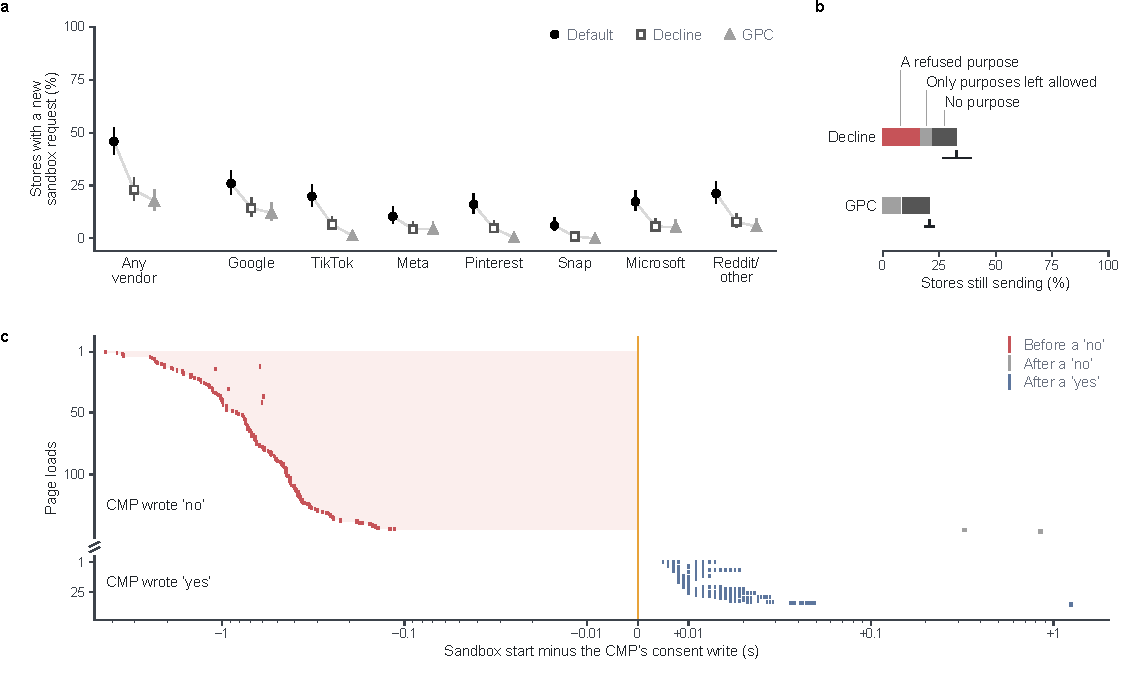
\includegraphics{fig5.pdf}
% GENERATED by paper/integrate_figures_v2.py from figures/v7/fig5/caption_fig5.tex (v2 figure caption, rendered by the figure script).
% Do not edit: change the figure script and re-run build.sh.
\caption{\textbf{A refusal stops new pixels that declare the refused purpose; pixels that started earlier, declare other purposes or declare none keep sending.}
(a)~The 231 stores where the Decline click worked, each loaded three ways: Default, and with a refusal (Decline, or the Global Privacy Control (GPC) signal). Share of stores on which a newly created sandbox (a Shopify web-pixel worker or iframe) sent an advertising request within 10~s, for any vendor and for each of the seven vendor groups. Any vendor: Default 106 of 231 (45.9\%; 95\% confidence interval (CI) 39.6--52.3); the fresh page after Decline 53 of 231 (22.9\%; 18.0--28.8); GPC 41 of 231 (17.7\%; 13.4--23.2). In every group Default is the highest of the three, and no store fired after Decline or under GPC without also firing under Default. Paired differences: Default $-$ Decline 22.9 percentage points (pp; 95\% CI 17.4--28.3); Default $-$ GPC 28.1~pp (22.2--33.9); Decline $-$ GPC 5.2~pp (0.2--10.3; 23 stores fired only after Decline and 11 only under GPC, exact McNemar $p = 0.058$). In each group the three loads of the same stores sit left to right in the arm coding of Fig.~S8a (filled black circle: Default; open dark-grey square: Decline; filled grey triangle: GPC; key at the top right), joined by a thin light-grey line, on the full percentage scale; the vendor groups are named on the x axis, with any vendor set apart on the left (per-vendor values, on the same scale: Fig.~S8a). Vertical lines: Wilson 95\% CIs; paired differences: Newcombe hybrid-score intervals.
(b)~Shopify's gate held the new pixels that declare the refused purpose (not drawn): after Decline, 0 of 196 stores had a new pixel declaring it; under GPC, 0 of 7,458 configured pixel entries that declare ``sale of data'' started (0 of 1,264 at-risk loads; 0 stores); while the region default denied ``marketing'', 2,206 of 2,234 entries that declare it were held (98.7\%; the other 28 started). The bars show what still got through: the share of stores that still sent a sandboxed ad request despite the refusal, Decline 64 of 196 (32.7\%; 95\% CI 26.5--39.5) and GPC 279 of 1,354 (20.6\%; 18.5--22.8). Each such store is in one class, assigned in the order a refused purpose, only purposes left allowed, no purpose; each thin bar stacks the classes from 0 in that order, and the classes are named once, at the Decline bar: a refused purpose (brick: a pixel that started before the refusal and declares the refused purpose kept sending, on the same page or in an unload beacon; Decline only, 32 stores), only purposes left allowed (grey; Decline 11, GPC 111), no purpose (dark grey; Decline 21, GPC 167). The greys of (b) mark these classes, not the arms of (a). Fig.~S8c uses the same class names, colours and order, by window and without the one-class-per-store rule. The GPC total includes 1 store that matched no class (not drawn). Decline: the 196 stores where Shopify recorded the refusal; GPC: the 1,354 stores where Shopify set ``sale of data: no''. Just under each bar: its total (a short tick rising toward the bar's end) on its Wilson 95\% CI (horizontal line).
(c)~The race between a consent-management platform (CMP) and pixel start-up: one row per page load in which a CMP wrote ``marketing: no'' to Shopify without a click (146 loads, 99 stores; upper block) or ``yes'' (35 loads, 23 stores; lower block); the row ticks count the loads within each block, so the row axis is broken between the blocks (cut marks). Each tick is one third-party sandbox that declares ``marketing'', at its start minus the CMP's consent write (amber line); rows are sorted by the load's first sandbox. The time axis is logarithmic on both sides of the write and linear between the two ticks nearest it, so that starts seconds before the write and milliseconds after it are both visible; every sandbox is drawn. The pale brick ground runs, row by row, from a ``no'' load's first sandbox to the write: the time its marketing sandboxes ran before the refusal arrived. Of the 535 sandboxes in the ``no'' loads, 525 started before the write (brick; median 653~ms before) and 10 after it (grey); all 342 in the ``yes'' loads started after it (slate; median 14~ms after); the key at the top right names the three tick colours. Throughout, brick marks consent lost (b, c), slate consent honoured (c), amber the consent moment (c) and grey context.}
\label{fig:choices}

\end{widefig}

Why does firing continue after a refusal that Shopify recorded? Figure~\ref{fig:choices}b classes each store once, and Supplementary Fig.~\ref*{S:fig:s8}c classes each residual sandboxed request by what its pixel declares and by Shopify's state at the time. New sandboxes of pixels declaring a refused purpose fired on none of the 196 stores: the gate held. Pixels started before the click that declare a refused purpose kept sending on 32 stores (16.3\%, 11.8--22.1\%), on the same page (19) or as unload beacons when the page reloaded (20), which any navigation away triggers (F3); their initiator stacks cannot separate events that Shopify delivered after the opt-out from the vendor's own timers. On 13 stores (6.6\%, 3.9--11.0\%) the pixel declared only purposes that the Decline had left allowed: CMPs recorded the Decline as a refusal of marketing, and sale of data stayed allowed on 112 of the 196 stores (F3, an incomplete refusal). On 28 stores (14.3\%, 10.1--19.9\%) the pixel declared no purpose (F4). Merchants' custom pixels were involved on 34 of the 37 stores with a fresh-page residual (Supplementary \ref*{S:sec:s-decline}).

\subsubsection{GPC}\label{sec:res-gpc}

Shopify honoured GPC: \code{saleOfDataAllowed()} was false in 1,166 of the 1,169 GPC loads with a readable state, and no configured pixel entry declaring sale of data started (0 of 7,458 entries in 1,264 loads at risk; upper 95\% bound 0.3\% of loads) or sent a request on any of the 1,354 stores where Shopify showed ``sale of data: no'' (Fig.~\ref{fig:choices}b). Yet of the 803 stores with a sandboxed ad request under Default, 279 (34.7\%, 31.5--38.1\%) still sent one under GPC: on 111 of the 1,354 stores from pixels declaring only purposes that GPC leaves allowed, mostly marketing (100), which Shopify's mapping of GPC to sale of data does not cover, and on 191 from pixels declaring no purpose (F4). Custom pixels alone accounted for the residual on 182 of the 279 stores.

Compared for persistence after the choice (the same 231 stores, new sandboxes on a later page, 10~s windows), a sandboxed ad request occurred on 53 stores after Decline and 41 under GPC (22.9\% and 17.7\%), a paired difference of 5.2 percentage points (95\% CI 0.2 to 10.3; exact McNemar $p=0.058$): GPC's advantage was between about 0 and 10 points. Over the whole visit the controls differ much more, because a Decline user is exposed before the click: a sandboxed ad request came before the click on 101 of these stores, against 41 over the whole GPC load (difference 26.0 percentage points, 95\% CI 20.0 to 31.7), although the pre-click window is the shorter. Counting attempted rather than working Declines changes little (Supplementary \ref*{S:sec:s-extended}).

\subsubsection{The gate held; the race was often lost}\label{sec:res-race}

To separate the gate from its inputs, we compared configured pixels at risk with the pixels that started. Beyond GPC (above), under a denying region default 2,206 of 2,234 marketing-declaring entries (98.7\%, 94.4--99.9\%, clustered by store) were held back in loads without a CMP ``yes''. Of 6,983 starts under a partly denied state by pixels that declare a purpose, 97 had a declared purpose denied at that moment; they came from 10 loads on 7 stores, so the rate to quote is per store, 7 of 1,179 (0.6\%, 0.3--1.2\%). Three of these loads were edge-cached pages carrying another region's consent string; the other seven we cannot explain (Supplementary \ref*{S:sec:s-gate}). Excluding the first pages of Decline loads, whose consent events were not recorded (Supplementary \ref*{S:sec:s-gate}), the gate held in almost all observed cases.

The state often arrived too late (Fig.~\ref{fig:choices}c; per load: Supplementary Fig.~\ref*{S:fig:s8}d). In 146 loads on 99 stores, a CMP wrote ``marketing: no'' to Shopify without any click; 525 of the 535 third-party sandboxes declaring marketing had already started when the write was dispatched, a median 653~ms earlier, and 291 of them before Shopify's consent script (\code{consent-tracking-api.js}) was even requested, a lower bound for any write through it. The first sandbox came first in 144 of the 146 loads. We found no code path by which the WPM terminates a started pixel; whether Shopify stopped delivering events to these pixels after the late ``no'' was not measured. Conversely, in 35 loads on 23 stores, mostly Pandectes stores, a CMP wrote ``marketing: yes'' without any click, in some cases (Pandectes' optional bot setting) because it detected an automated browser, and all 342 gated third-party sandboxes started after it. Practitioners have described this race \citep{analyticsninja2025pixels,weltpixel2026race}; to our knowledge these are the first measurements of how often it happens.

% ----------------------------------------------------------------------------
\subsection{Beyond Shopify: a pilot}\label{sec:res-beyond}
% ----------------------------------------------------------------------------

The Round 4 crawl also loaded, with the same three arms, sites on two other hosted commerce platforms and sites that send tags through a first-party gateway (Section~\ref{sec:method-r4}; Supplementary Fig.~\ref*{S:fig:s10}). These are selected sites, not samples of a population, and an ad request here also counts a first-party request whose wire format names Google Ads, Meta or TikTok. Before any choice, an ad request left the page on 28 of 57 Wix, 48 of 72 BigCommerce and 17 of 19 gateway sites that showed a banner. After a working Decline, ad requests continued on 14 of 33 Wix sites (42.4\%, 27.2--59.2\%), 32 of 53 BigCommerce sites (60.4\%, 46.9--72.4\%) and 7 of 8 gateway sites. GPC made little difference, and Partytown and Cloudflare Zaraz were too rare for rates (details: Supplementary \ref*{S:sec:s-r4} and~\ref*{S:sec:s-extended}). A browser cannot see what a gateway forwards on the server side, so the gateway results are lower bounds on what vendors receive.
